%
% Modelo LaTeX baseado no modelo A5L
% Adaptação para LaTeX por Bruno Ferreira

% Nota: usar /newpage com 1 coluna
%       usar /clearpage com 2 colunas
%       o /newpage com duas colunas escreve na próxima coluna
\documentclass[a5paper,twocolumn, 11pt]{article}
\usepackage[landscape]{geometry}

%Sample text
%\usepackage{lipsum}

%escrever acentos e coisas do género sem que o latex se desoriente
\usepackage[utf8]{inputenc}

%hifenização e titulos em português
\usepackage[portuges]{babel}

%para ter a informação de quantas páginas tem o documento
\usepackage{lastpage}

%importar cores predefinidas
\usepackage[usenames,dvipsnames]{xcolor}
\definecolor{DarkGray}{gray}{0.40}

%usar multirow e multicolumn
\usepackage{multirow}

%para ter imagens, depois define a directoria de imagens
\usepackage{graphicx}
\graphicspath{{./imagens/}}

%poder ter texto sublinhado que passa para a linha seguinte automaticamente
%usar com \uline{my underline text}
\usepackage[normalem]{ulem}

%definir o cabeçalho e rodapé
\usepackage{fancyhdr}
\pagestyle{fancy}
\fancyhead[L]{
    \small{
        \textcolor{DarkGray}{
            \textbf{Uminho 2012 - LI3 --- Transitários LEI}
        }
    }
}
\fancyhead[R]{
    \small{
        \textcolor{DarkGray}{
            \textbf{Pág. \thepage\ /\pageref{LastPage}}
        }
    }
}
\fancyfoot[C]{}

%definir regras de hifenização
\hyphenation{
chaining
Hash
}

%definir comando \hyph{}, necessário para n\hyph{}dimensionais
\def\hyph{-\penalty0\hskip0pt\relax}

\begin{document}

\onecolumn
\thispagestyle{empty}
\begin{tabular}{ll}
    \multirow{7}{*}{ 
\includegraphics[height=90pt]{logo.jpeg} }
    &\\
    & \textcolor{DarkGray}{\Large{\textbf{Escola de Engenharia}}} \\
    &\\
    & \large{Departamento de Informática}\\
    &\\
    &\\
    & \large{Licenciatura em Engenharia Informática}\\
\end{tabular}
\begin{center}
    \Large{\textbf{Projecto de Laboratórios de Informática III}}\\
    \vspace{20pt}
    \Large{\textbf{``Transistários LEI --- Projecto 2: Parte I''}}\\
    \vspace{15pt}
    \begin{tabular}{r@{, }l}
        Bruno Ferreira&A61055\\
        Daniel Carvalho&A61008\\
    \end{tabular}
    
    \vspace{5pt}
    \emph{Grupo 42}\\\vspace{15pt}
    \large{\textbf{Braga, Maio de 2012}}
\end{center}

\newpage
\twocolumn
\tableofcontents
\newpage
\listoffigures

\newpage
\section{Resumo}
Neste relatório encontram-se explicitados dados relativos ao desempenho do uso de colecções de Java para o mesmo tipo de problema do projecto anterior realizado nesta unidade curricular. Tem-se como objectivo medir o desempenho das várias colecções aplicadas aos mesmos dados de forma a ser possível recolher informação que permita avaliar e obter conclusões concretas relativamente às vantagens e desvantagens de cada uma das ditas colecções. O factor de medição é o tempo despendido nas operações implementadas para as diversas colecções a avaliar. A avaliação do desempenho das colecções a usar segue neste relatório com o suporte de gráficos e análises estatísticas como a média e o desvio padrão.
Na medição de desempenho são feitas 10 medições para várias grandezas de informação, dessa forma é possível proceder à análise dos dados com a garantia de alguma fiabilidade.

\clearpage
\section{Introdução}
De forma a comparar o desempenho entre as estruturas de dados usadas no primeiro projecto e aquelas que podem ser usadas em Java são registados os tempos das operações que serão enunciadas de seguida tendo em conta a  estrutura de utilizadores e localidades. Para as operações são considerados diferentes patamares de número de elementos: 5000, 10000, 15000, 18000.

Todo o código foi criado de forma a reflectir, com realismo, os valores de desempenho da utilização das diferentes colecções numa aplicação real. Assim, processos como a clonagem de objectos, a verificação de repetidos e a verificação da existência da localidade de destino antes da inserção de ligações foram implementadas e incluídas nas cronometragens.

As operações sobre utilizadores a efectuar são:
\begin{enumerate}
    \item{carregar base de dados de utilizadores a partir de um ficheiro;}
    \item{inserir o registo de um novo utilizador;}
    \item{procurar um utilizador por nome e nif;}
    \item{percorrer (visitar) a estrutura e imprimir os dados dos utilizadores.}
\end{enumerate}

As operações sobre localidades a efectuar são:
\begin{enumerate}
    \item{carregar base de dados de localidades e ligações a outras localidades a
partir de um ficheiro;}
    \item{inserir o registo de uma nova localidade;}
    \item{inserir o registo de uma nova ligação a uma localidade;}
    \item{procurar as ligações de uma localidade;}
    \item{percorrer (visitar) a estrutura e imprimir os dados das localidades.}
\end{enumerate}

No que respeita às diferentes configurações para a estrutura de dados sobre utilizadores, são testadas e registadas informações relativas ao desempenho de:
\begin{enumerate}
    \item{duas estruturas baseadas em ArrayList para fazer a ordenação pelos
dois critérios: nome e nif;}
    \item{uma estrutura baseada em ArrayList para fazer a ordenação por nome
e uma estrutura auxiliar em LinkedList para a ordenação por nif;}
    \item{duas estruturas baseadas em HashMap, para guardar dados ordenados dos utilizadores;}
    \item{duas estruturas baseadas em TreeMap, para guardar dados ordenados dos utilizadores;}
\end{enumerate}

No que respeita às diferentes configurações para a estrutura de dados sobre localidades, são testadas e registadas informações relativas ao desempenho de:
\begin{enumerate}
    \item{uma estrutura baseada em ArrayList para fazer a gestão das localidades e um ArrayList para as localidades relacionadas;}
    \item{uma estrutura baseada em ArrayList para fazer a gestão das localidades e um HashSet para as localidades relacionadas;}
    \item{uma estrutura baseada em HashMap para localidades com um HashMap
para as localidades relacionadas;}
    \item{uma estrutura baseada em TreeMap para localidades com um TreeMap
para as localidades relacionadas.}
\end{enumerate}
\clearpage
\newpage
\section{Conteúdo}
\subsection{O ambiente de testes}

A resolução do relógio usado (tempo mínimo que o cronómetro consegue cronometrar) é de 1 milisegundo. Então recorreu-se à execução de 400 repetições dos procedimentos de inserção de informação e de pesquisa de informação, visto que uma execução dessas operações demoraria menos de 1 milisegundo. Desta forma é possível obter valores médios com maior exactidão.

Assim, note-se ainda que na fase de impressão não são imprimidos 5000, 10000, 15000 ou 18000 valores no ecrã, devido aos 400 valores extra que são inseridos para poder obter valores respeitantes aos tempos de inserção.

De forma a uniformizar os resultados, todos os testes foram efectuados na mesma máquina. As especificações técnicas dessa máquina são as seguintes:\\
\\
\begin{tabular}{ | r  | p{2.8cm} | }
    \hline
    Sistema Operativo: & Windows 7 64bit \\
    Modelo: & Acer BA50-MV \\
    Processador: & \vbox{Intel Pentium} T4400 \vbox{Dual-Core} @ 2.2GHz \\
    Caches: & \vbox{L1-D 2x32Kb}
    \vbox{L1-I 2x32Kb}
    \vbox{L2 1024Kb} \\
    RAM: & 2x2048MB DDR3 533MHz\\ \hline
\end{tabular}\\
\\

Relembra-se que cada um destes testes é efectuado para diferentes patamares de número de elementos: 5000, 10000, 15000, 18000.\\

Para facilitar o uso das diferentes configurações de estrutura de dados é usada uma classe abstracta de Utilizadores (que gere as várias colecções de utilizadores). Assim, ao aumentar o nível de abstracção sobre a classe de utilizadores, é possível obter uma implementação mais genérica e legível. Também existe abstracção nas classes Localidades (que gere uma colecção de localidades) e Ligações (que gere uma colecção de ligações entre a localidade actual e uma qualquer outra localidade).
Com este tipo de implementação, o código de medição de tempos é simplificado, pois existe uma camada extra de abstracção que permite que as várias estruturas de dados sejam tratadas de igual forma. O método anteriormente descrito também simplifica as funções de inserção de dados a partir de ficheiros.
\subsubsection{Utilizadores}
Os testes sobre utilizadores têm o padrão de execução descrito em seguida.

Inicialmente é executada uma vez o seguinte conjunto de operações:
\begin{enumerate}
    \item ler utilizadores do ficheiro e inseri-los na estrutura de dados;
    \item inserir dados de teste (400 dados que não representam nada em concreto, mas que são necessários para contornar as limitações do relógio usado);
    \item pesquisar por NIF e por nome;
    \item escrever utilizadores para ficheiro.
\end{enumerate}
Após esta fase inicial (warm\hyph{}up), o conjunto de operações é executado dez vezes e através dessa execução são obtidos valores da cronometragem de cada operação. Destes últimos conseguem-se retirar valores como o tempo médio e desvio padrão.\\
\subsubsection{Localidades}
Os testes sobre localidades são executados da seguinte forma.

Inicialmente é executada uma vez o seguinte conjunto de operações:
\begin{enumerate}
    \item ler localidades e ligações do ficheiro e povoar as estruturas com os dados lidos;
    \item inserir dados de teste (400 dados que não representam nada em concreto, mas que são necessários para contornar as limitações do relógio usado);
    \item pesquisar todas as ligações de cada localidade;
    \item imprimir informações de localidades.
\end{enumerate}

Após esta fase inicial (warm\hyph{}up), o conjunto de operações é executado dez vezes e através dessa execução são obtidos valores da cronometragem de cada operação. Destes últimos conseguem-se retirar valores como o tempo médio e desvio padrão.

\clearpage
\subsection{Estatísticas}
No seguimento deste relatório constam informações individuais e detalhadas sobre o desempenho das operações efectuadas sobre utilizadores e localidades nas diversas configurações da estrutura de dados.

Todos os gráficos apresentados, à excepção dos gráficos de comparação de resultados, têm uma representação do desvio padrão. Os losangos a preto unidos por uma linha que se encontram aos 5000, 10000, 15000 e 18000 resultados, delimitam os valores no conjunto $[\mu-\sigma; \mu+\sigma]$ que correspondem a $68.2\%$ dos tempos.

Todos os gráficos são acompanhados de uma tabela com valores mais precisos das avaliações de desempenho.


\subsubsection{Utilizadores: ArrayList}
Utilizar dois ArrayList para guardar os Utilizadores (sendo que um deles está ordenado por número de contribuinte ou NIF e o outro está ordenado por nome) é ineficiente comparado com as outras configurações.

Os tempos de leitura e inserção de dados crescem exponencialmente, significando que, embora pareça uma solução aceitável até às 5000 inserções, torna-se extremamente ineficiente para uma quantidade de dados superior a poucos milhares.

Os tempos de pesquisa têm um crescimento linear, assim sendo não é muito ineficiente. A escrita segue o mesmo modelo e também não é muito ineficiente.
\clearpage
\onecolumn
\begin{center}
    \begin{table}[h!b!t!]
    \begin{center}
    \caption{Tempos da configuração ArrayList}
    \begin{tabular}[hbt]{ | *{11}{c|} }
    \hline
        Num. & \multicolumn{2}{|c|}{ler ficheiro} & \multicolumn{2}{|c|}{inserir}\\ %\hline
        Dados & $\mu$ & $\sigma$ & $\mu$ & $\sigma$\\ \hline
        5000 & 956.6 & 40.37 & 79.2 & 10.32\\ \hline
        10000 & 6246.7 & 747.47 & 467.8 & 104.56\\ \hline
        15000 & 23116.9 & 3171.60 & 1204.2 & 131.06\\ \hline
        18000 & 43571.1 & 5503.52 & 1582.8 & 415.43\\ \hline
    \end{tabular}
\end{center}
\end{table}
    \begin{tabular}{ | *{11}{c|} }
    \hline
        Num.  & \multicolumn{2}{|c|}{pesquisar nome} & \multicolumn{2}{|c|}{pesquisar nif} & \multicolumn{2}{|c|}{escrever}\\ %\hline
        Dados & $\mu$ & $\sigma$ & $\mu$ & $\sigma$ & $\mu$ & $\sigma$\\ \hline
        5000 & 21.2 & 2.14 & 956.6 & 40.37 & 79.2 & 10.32\\ \hline
        10000 & 129.9 & 28.19 & 6246.7 & 747.47 & 467.8 & 104.56\\ \hline
        15000 & 401.8 & 59.72 & 23116.9 & 3171.60 & 1204.2 & 131.06\\ \hline
        18000 & 556.0 & 139.33 & 43571.1 & 5503.52 & 1582.8 & 415.43\\ \hline
    \end{tabular}
\end{center}
\begin{figure}[h!b!t!]
    \caption[Utilizadores: ArrayList (ler de ficheiro)]{Utilizadores: ArrayList (ler de ficheiro).}
    \label{hashtable}
    \centering
        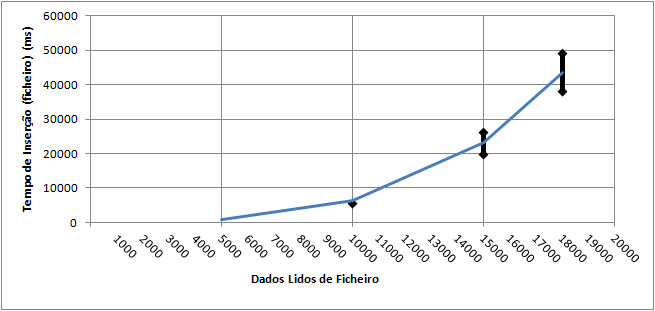
\includegraphics[width=400pt]{user_c1_o1.png}
\end{figure}
\begin{figure}[h!b!t!]
    \caption[Utilizadores: ArrayList (inserir dados gerados)]{Utilizadores: ArrayList (inserir dados gerados).}
    \label{hashtable}
    \centering
        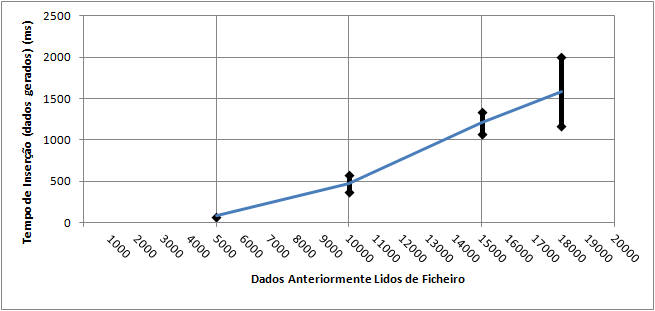
\includegraphics[width=400pt]{user_c1_o2.png}
\end{figure}
\begin{figure}[h!b!t!]
    \caption[Utilizadores: ArrayList (pesquisar por nome)]{Utilizadores: ArrayList (pesquisar por nome).}
    \label{hashtable}
    \centering
        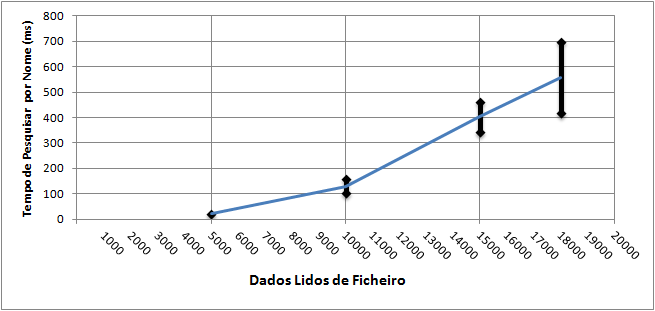
\includegraphics[width=400pt]{user_c1_o3.png}
\end{figure}
\begin{figure}[h!b!t!]
    \caption[Utilizadores: ArrayList (pesquisar por nif)]{Utilizadores: ArrayList (pesquisar por nif).}
    \label{hashtable}
    \centering
        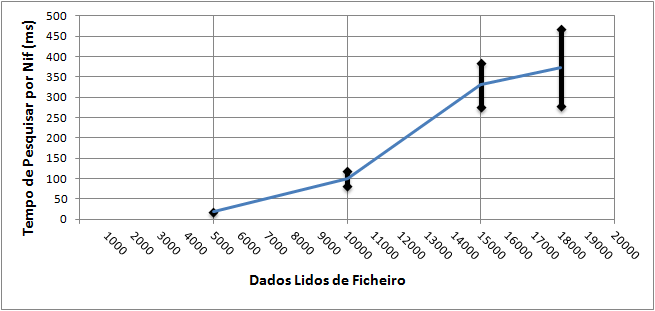
\includegraphics[width=400pt]{user_c1_o4.png}
\end{figure}
\begin{figure}[h!b!t!]
    \caption[Utilizadores: ArrayList (imprimir dados)]{Utilizadores: ArrayList (imprimir dados).}
    \label{hashtable}
    \centering
        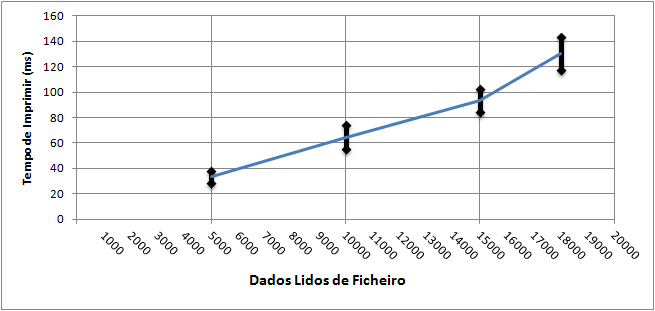
\includegraphics[width=400pt]{user_c1_o5.png}
\end{figure}

\newpage
\twocolumn
\subsubsection[Utilizadores:\\ArrayList e LinkedList]{Utilizadores: \vbox{ArrayList e LinkedList}}
Utilizar um ArrayList para guardar os Utilizadores ordenados por nif e um LinkedList para guardar os mesmos dados ordenados por nome, é ainda mais ineficiente que usar 2 arraylist.

Os tempos são extremamente altos no que diz respeito às inserções, além disso são variações na forma exponencial, logo tendem a crescer ainda mais.
Quanto às outras variações, estas assumem uma forma mais próxima do linear.

\clearpage
\onecolumn
\begin{center}
    \begin{table}[h!b!t!]
    \begin{center}
    \caption{Tempos da configuração ArrayList e LinkedList}
\begin{tabular}{ | *{11}{c|} }
\hline
    Num. & \multicolumn{2}{|c|}{ler ficheiro} & \multicolumn{2}{|c|}{inserir}\\ %\hline
    
    Dados & $\mu$ & $\sigma$ & $\mu$ & $\sigma$\\ \hline
    5000 & 37780.2 & 440.90 & 15308.1 & 57.65\\ \hline
    10000 & 332729.7 & 36485.49 & 60034.0 & 12987.33\\ \hline
    15000 & 1195102.1 & 117008.82 & 149284.1 & 11049.01\\ \hline
    18000 & 2144097.5 & 5194.45 & 222223.5 & 647.58\\ \hline
\end{tabular}
\end{center}
\end{table}
\begin{tabular}{ | *{11}{c|} }
\hline
    Num. & \multicolumn{2}{|c|}{pesquisar nome} & \multicolumn{2}{|c|}{pesquisar nif} & \multicolumn{2}{|c|}{escrever}\\ %\hline
    
    Dados & $\mu$ & $\sigma$ & $\mu$ & $\sigma$ & $\mu$ & $\sigma$\\ \hline
    5000 & 51.7 & 43.45 & 23.0 & 13.84 & 32.1 & 5.32\\ \hline
    10000 & 255.6 & 114.50 & 124.1 & 83.08 & 64.8 & 9.70\\ \hline
    15000 & 581.4 & 55.20 & 294.1 & 16.80 & 116.1 & 15.36\\ \hline
    18000 & 767.5 & 20.35 & 408.5 & 10.65 & 141.7 & 17.46\\ \hline
\end{tabular}
\end{center}

\begin{figure}[h!b!t!]
    \caption[Utilizadores: ArrayList e Linked List (ler de ficheiro)]{Utilizadores: ArrayList e LinkedList (ler de ficheiro).}
    \label{hashtable}
    \centering
        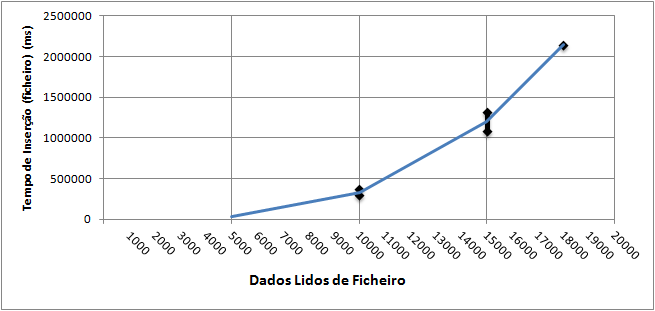
\includegraphics[width=400pt]{user_c2_o1.png}
\end{figure}
\begin{figure}[h!b!t!]
    \caption[Utilizadores: ArrayList e Linked List (inserir dados gerados)]{Utilizadores: ArrayList e LinkedList (inserir dados gerados).}
    \label{hashtable}
    \centering
        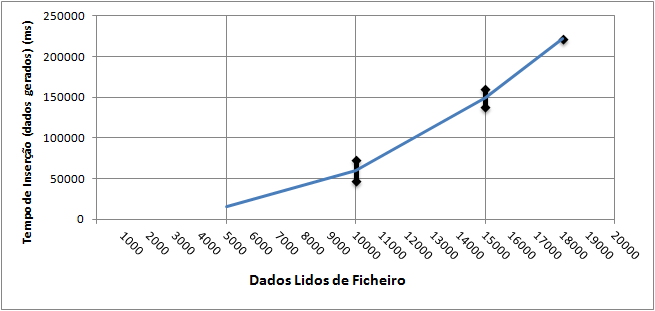
\includegraphics[width=400pt]{user_c2_o2.png}
\end{figure}
\begin{figure}[h!b!t!]
    \caption[Utilizadores: ArrayList e Linked List (pesquisar por nome)]{Utilizadores: ArrayList e LinkedList (pesquisar por nome).}
    \label{hashtable}
    \centering
        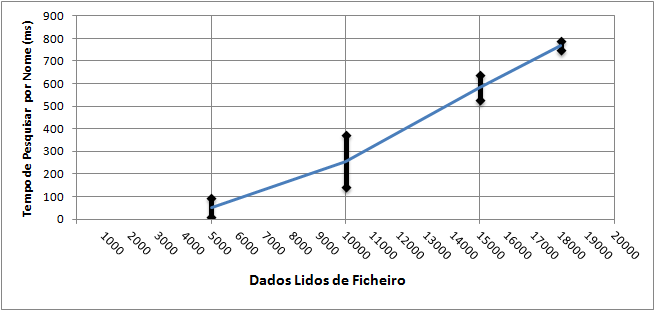
\includegraphics[width=400pt]{user_c2_o3.png}
\end{figure}
\begin{figure}[h!b!t!]
    \caption[Utilizadores: ArrayList e Linked List (pesquisar por nif)]{Utilizadores: ArrayList e LinkedList (pesquisar por nif).}
    \label{hashtable}
    \centering
        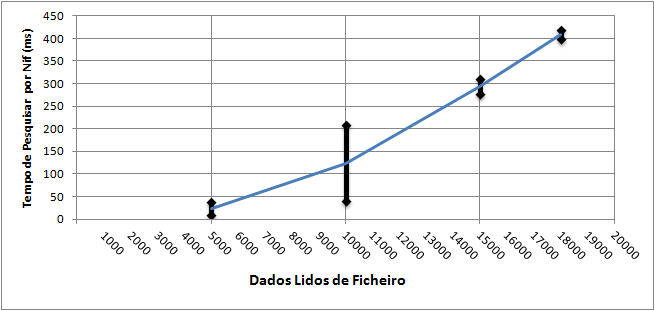
\includegraphics[width=400pt]{user_c2_o4.png}
\end{figure}
\begin{figure}[h!b!t!]
    \caption[Utilizadores: ArrayList e Linked List (imprimir dados)]{Utilizadores: ArrayList e LinkedList (imprimir dados).}
    \label{hashtable}
    \centering
        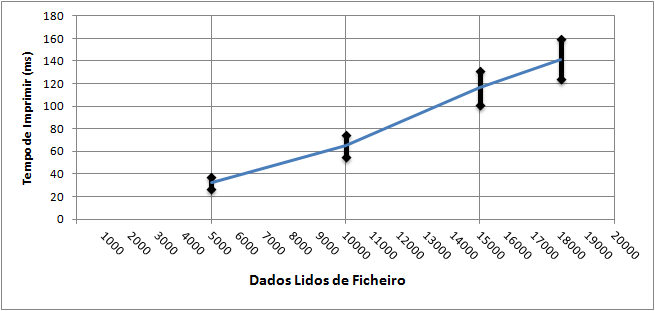
\includegraphics[width=400pt]{user_c2_o5.png}
\end{figure}

\newpage
\twocolumn
\subsubsection{Utilizadores: HashMap}
Ter 2 HashMap (cujas chaves são o número de contribuinte e o nome, respectivamente) é uma solução excelente.
A variação dos tempos de inserção aproxima a forma logarítmica, e as pesquisas aproximam uma recta constante e muito próxima de 0ms.
O problema do HashMap é a sua travessia ``não natural'', que, por ser uma implementação de força bruta, demora, em média, um pouco mais que as outras operações. A impressão dos dados com HashMap segue uma variação linear.

Assim sendo, está é a melhor solução até agora, mesmo com a pequena desvantagem da impressão à base de força bruta.
\clearpage
\onecolumn
    \begin{table}[h!b!t!]
    \begin{center}
    \caption{Tempos da configuração HashMap}
\begin{tabular}{ | *{11}{c|} }
\hline
    Num. & \multicolumn{2}{|c|}{ler ficheiro} & \multicolumn{2}{|c|}{inserir} & \multicolumn{2}{|c|}{pesquisar nome} & \multicolumn{2}{|c|}{pesquisar nif} & \multicolumn{2}{|c|}{escrever}\\ %\hline
    
    Dados & $\mu$ & $\sigma$ & $\mu$ & $\sigma$ & $\mu$ & $\sigma$ & $\mu$ & $\sigma$ & $\mu$ & $\sigma$\\ \hline
    5000 & 5.3 & 1.70 & 0.2 & 0.42 & 0.5 & 0.97 & 0.1 & 0.31 & 35.0 & 4.69\\ \hline
    10000 & 10.2 & 2.65 & 0.0 & 0.0 & 0.2 & 0.42 & 0.0 & 0.0 & 67.1 & 6.93\\ \hline
    15000 & 14.4 & 1.07 & 0.1 & 0.31 & 0.6 & 1.89 & 0.0 & 0.0 & 94.5 & 7.74\\ \hline
    18000 & 14.9 & 0.56 & 0.1 & 0.31 & 0.0 & 0.0 & 0.0 & 0.0 & 123.0 & 12.66\\ \hline
\end{tabular}
\end{center}
\end{table}

\begin{figure}[h!b!t!]
    \caption[Utilizadores: HashMap (ler de ficheiro)]{Utilizadores: HashMap (ler de ficheiro).}
    \label{hashtable}
    \centering
        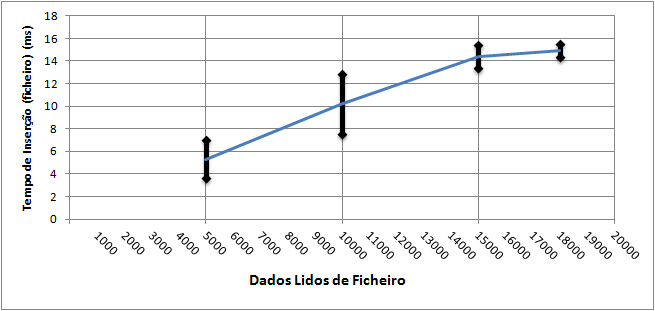
\includegraphics[width=400pt]{user_c3_o1.png}
\end{figure}
\begin{figure}[h!b!t!]
    \caption[Utilizadores: HashMap (inserir dados gerados)]{Utilizadores: HashMap (inserir dados gerados).}
    \label{hashtable}
    \centering
        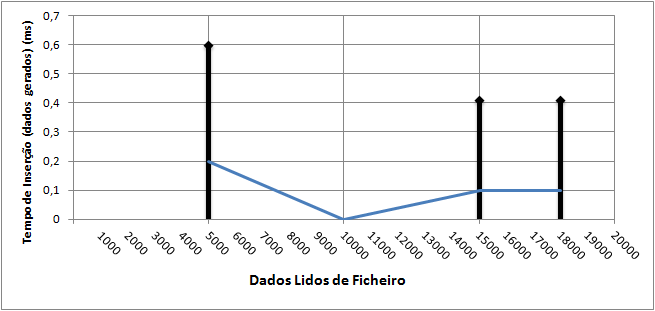
\includegraphics[width=400pt]{user_c3_o2.png}
\end{figure}
\begin{figure}[h!b!t!]
    \caption[Utilizadores: HashMap (pesquisar por nome)]{Utilizadores: HashMap (pesquisar por nome).}
    \label{hashtable}
    \centering
        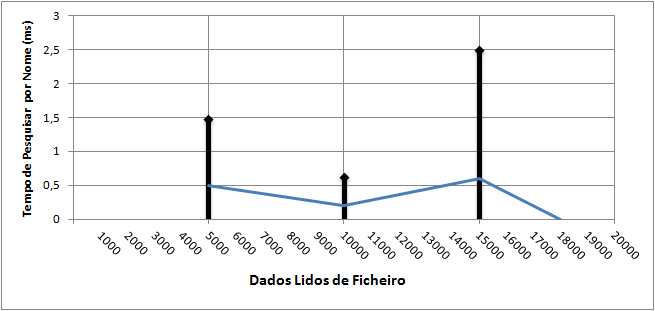
\includegraphics[width=400pt]{user_c3_o3.png}
\end{figure}
\begin{figure}[h!b!t!]
    \caption[Utilizadores: HashMap (pesquisar por nif)]{Utilizadores: HashMap (pesquisar por nif).}
    \label{hashtable}
    \centering
        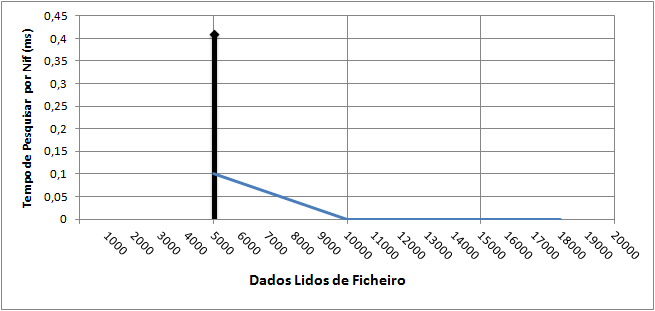
\includegraphics[width=400pt]{user_c3_o4.png}
\end{figure}
\begin{figure}[h!b!t!]
    \caption[Utilizadores: HashMap (imprimir dados)]{Utilizadores: HashMap (imprimir dados).}
    \label{hashtable}
    \centering
        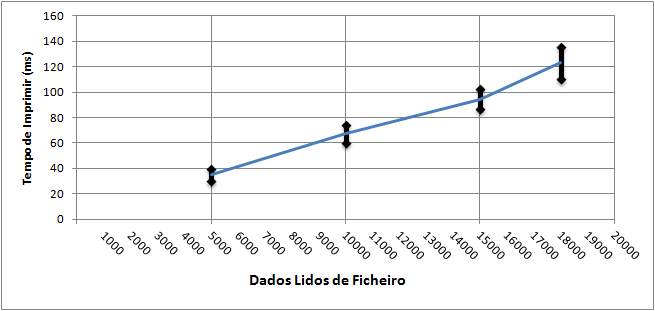
\includegraphics[width=400pt]{user_c3_o5.png}
\end{figure}

\newpage
\twocolumn
\subsubsection{Utilizadores: TreeMap}
Ter 2 TreeMap (cujas chaves são o número de contribuinte e o nome, respectivamente) é uma excelente solução.
A variação dos tempos de inserção aproxima a forma linear, e as pesquisas aproximam uma recta constante e muito próxima de 0ms.
A variação do tempo de impressão dos dados aproxima a forma linear.

Assim sendo, está é uma das melhores soluções para trabalhar os dados relativos a utilizadores.

\clearpage
\onecolumn
    \begin{table}[h!b!t!]
    \begin{center}
    \caption{Tempos da configuração TreeMap}
\begin{tabular}{ | *{11}{c|} }
\hline
    Num. & \multicolumn{2}{|c|}{ler ficheiro} & \multicolumn{2}{|c|}{inserir} & \multicolumn{2}{|c|}{pesquisar nome} & \multicolumn{2}{|c|}{pesquisar nif} & \multicolumn{2}{|c|}{escrever}\\ %\hline
    
    Dados & $\mu$ & $\sigma$ & $\mu$ & $\sigma$ & $\mu$ & $\sigma$ & $\mu$ & $\sigma$ & $\mu$ & $\sigma$\\ \hline
    5000 & 14.7 & 5.53 & 1.1 & 2.80 & 0.1 & 0.31 & 0.2 & 0.42 & 41.0 & 14.81\\ \hline
    10000 & 24.3 & 0.48 & 0.6 & 0.51 & 0.0 & 0.0 & 0.1 & 0.31 & 62.5 & 2.75\\ \hline
    15000 & 40.4 & 2.45 & 0.5 & 0.52 & 0.0 & 0.0 & 0.0 & 0.0 & 92.5 & 5.54\\ \hline
    18000 & 48.2 & 0.63 & 0.8 & 0.42 & 0.0 & 0.0 & 0.1 & 0.31 & 116.7 & $5.75$\\ \hline
    
\end{tabular}
\end{center}
\end{table}

\begin{figure}[h!b!t!]
    \caption[Utilizadores: TreeMap (ler de ficheiro)]{Utilizadores: TreeMap (ler de ficheiro).}
    \label{hashtable}
    \centering
        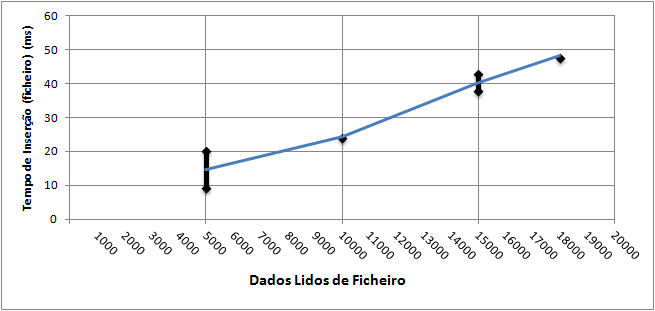
\includegraphics[width=400pt]{user_c4_o1.png}
\end{figure}
\begin{figure}[h!b!t!]
    \caption[Utilizadores: TreeMap (inserir dados gerados)]{Utilizadores: TreeMap (inserir dados gerados).}
    \label{hashtable}
    \centering
        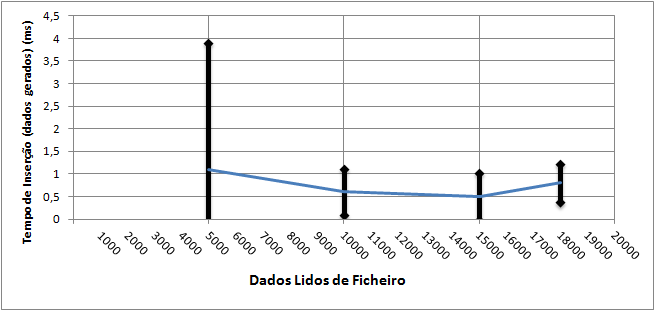
\includegraphics[width=400pt]{user_c4_o2.png}
\end{figure}
\begin{figure}[h!b!t!]
    \caption[Utilizadores: TreeMap (pesquisar por nome)]{Utilizadores: TreeMap (pesquisar por nome).}
    \label{hashtable}
    \centering
        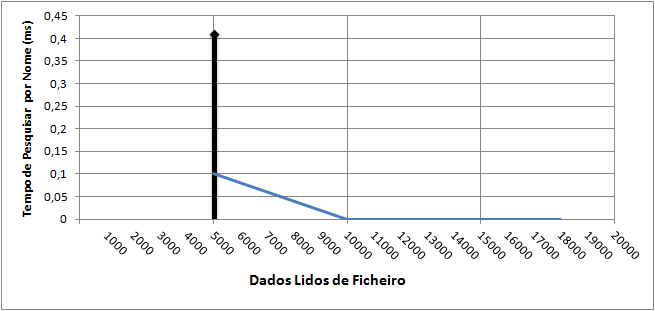
\includegraphics[width=400pt]{user_c4_o3.png}
\end{figure}
\begin{figure}[h!b!t!]
    \caption[Utilizadores: TreeMap (pesquisar por nif)]{Utilizadores: TreeMap (pesquisar por nif).}
    \label{hashtable}
    \centering
        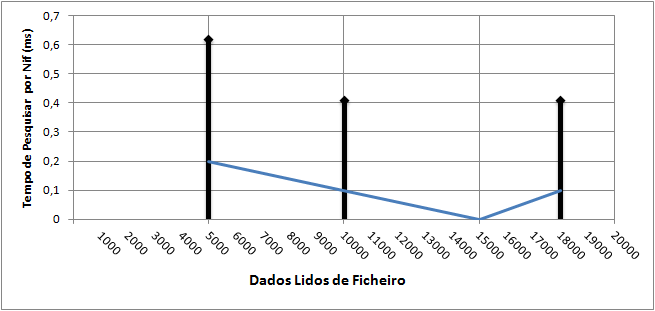
\includegraphics[width=400pt]{user_c4_o4.png}
\end{figure}
\begin{figure}[h!b!t!]
    \caption[Utilizadores: TreeMap (imprimir dados)]{Utilizadores: TreeMap (imprimir dados).}
    \label{hashtable}
    \centering
        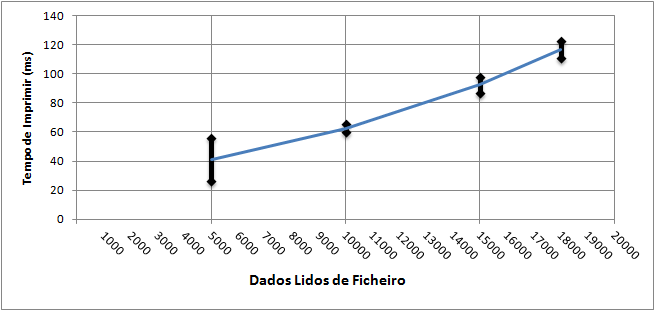
\includegraphics[width=400pt]{user_c4_o5.png}
\end{figure}




\newpage
\twocolumn
\newpage

\subsubsection[Utilizadores:\\Comparação]{Utilizadores: Comparação}
Como já foi antes visto (e pode ser verificado pela observação dos gráficos que comparam as várias configurações, abaixo), usar a configuração de 2 ArrayList é mau, e usar a configuração de ArrayList com um LinkedList auxiliar é ainda pior.

Ficam então o HashMap e o TreeMap.

A vantagem natural de uma árvore face a uma tabela de procura é a possibilidade de poder percorrer todos os nodos de uma árvore. Isto porque segundo o conceito de tabela de procura, esta só pode ser iterada usando um método de força-bruta, que obriga a percorrer todas as posições da tabela de procura, mesmo as que não têm interesse.
A grande desvantagem da árvore é a forma muito complexa como os nodos são inseridos na árvore, que obriga a uma grande quantidade de cálculos para que a árvore se mantenha balanceada.

Ao observar de novo os gráficos relativos à implementação de HashMap e de TreeMap, conclui-se que o tempo ganho ao usar HashMap (que tem maior vantagem na inserção) é bastante superior ao TreeMap (que apenas tem uma pequena vantagem face ao HashMap no que diz respeito à iteração).

Assim sendo, conclui-se que a implementação de 2 HashMap é melhor que qualquer outra das implementações cronometradas.

\clearpage
\onecolumn
\begin{figure}[h!b!t!]
    \caption[Utilizadores: Comparação (ler de ficheiro)]{Utilizadores: Comparação (ler de ficheiro).}
    \label{hashtable}
    \centering
        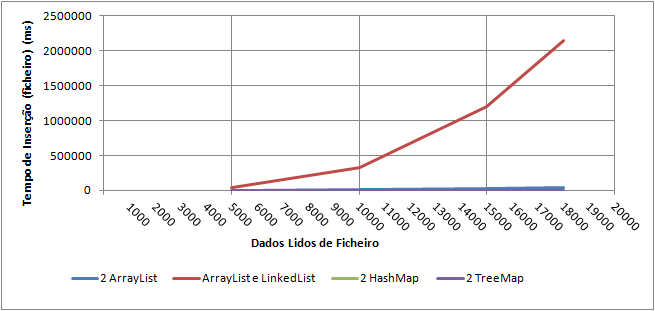
\includegraphics[width=400pt]{cusers_o1.png}
\end{figure}
\begin{figure}[h!b!t!]
    \caption[Utilizadores: Comparação (inserir dados gerados)]{Utilizadores: Comparação (inserir dados gerados).}
    \label{hashtable}
    \centering
        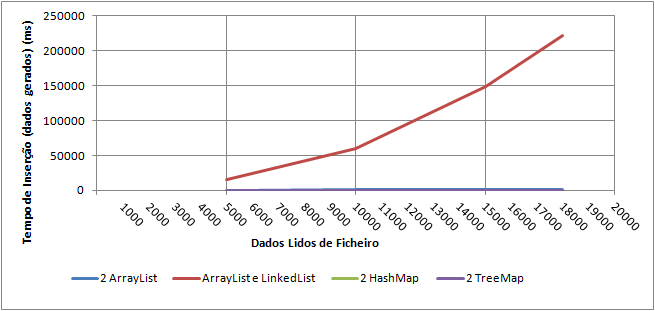
\includegraphics[width=400pt]{cusers_o2.png}
\end{figure}
\begin{figure}[h!b!t!]
    \caption[Utilizadores: Comparação (pesquisar por nome)]{Utilizadores: Comparação (pesquisar por nome).}
    \label{hashtable}
    \centering
        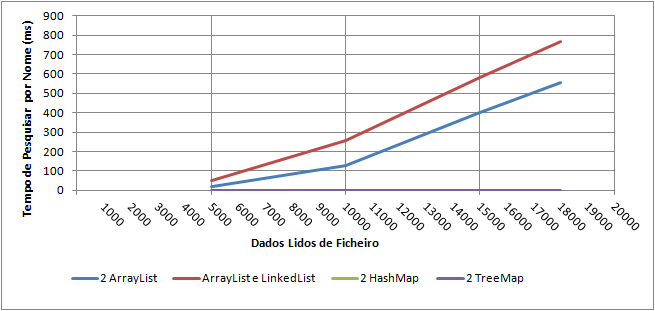
\includegraphics[width=400pt]{cusers_o3.png}
\end{figure}
\begin{figure}[h!b!t!]
    \caption[Utilizadores: Comparação (pesquisar por nif)]{Utilizadores: Comparação (pesquisar por nif).}
    \label{hashtable}
    \centering
        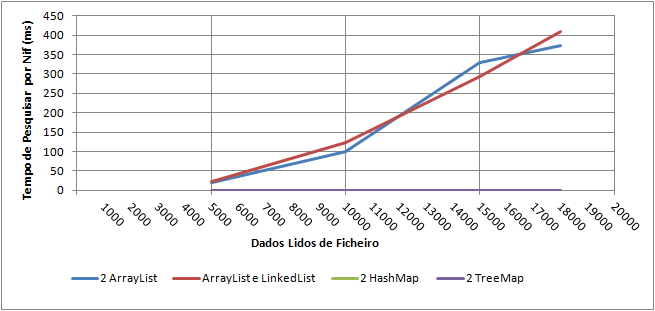
\includegraphics[width=400pt]{cusers_o4.png}
\end{figure}
\begin{figure}[h!b!t!]
    \caption[Utilizadores: Comparação (imprimir dados)]{Utilizadores: Comparação (imprimir dados).}
    \label{hashtable}
    \centering
        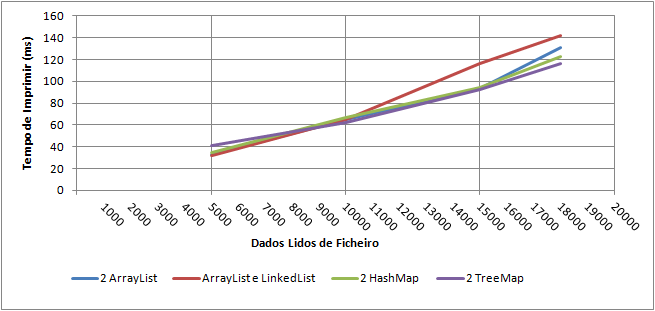
\includegraphics[width=400pt]{cusers_o5.png}
\end{figure}

\twocolumn
\newpage














\subsubsection{Localidades: ArrayList}
A implementação de 2 ArrayList para manusear dados relativos a localidades é uma solução extremamente lenta, independentemente de ser, ou não, eficiente.

Aparentemente, os tempos das inserções a partir de um ficheiro seguem uma norma exponencial, mas depois verifica-se, ao inserir valores com base nos dados gerados pelo programa, que a variação de tempo destes últimos aproxima a forma linear.

A variação dos tempos de impressão dos dados segue uma forma exponencial.
\clearpage
\onecolumn
\begin{center}
    \begin{table}[h!b!t!]
    \begin{center}
    \caption{Tempos da configuração ArrayList}
    \begin{tabular}[hbt]{ | *{11}{c|} }
    \hline
        Num. & \multicolumn{2}{|c|}{ler ficheiro} & \multicolumn{2}{|c|}{inserir localidades}\\ %\hline
        Dados & $\mu$ & $\sigma$ & $\mu$ & $\sigma$\\ \hline
        5000 & 17144.5 & 1071.13 & 30.6 & 3.77\\ \hline
        10000 & 53844.0 & 12886.71 & 88.0 & 23.21\\ \hline
        15000 & 119427.3 & 34189.41 & 332.3 & 66.22\\ \hline
        18000 & 169829.5 & 70858.03 & 254.0 & 162.76\\ \hline
    \end{tabular}
\end{center}
\end{table}
    \begin{tabular}{ | *{11}{c|} }
    \hline
        Num.  & \multicolumn{2}{|c|}{inserir ligações} & \multicolumn{2}{|c|}{pesquisar ligações} & \multicolumn{2}{|c|}{escrever}\\ %\hline
        Dados & $\mu$ & $\sigma$ & $\mu$ & $\sigma$ & $\mu$ & $\sigma$\\ \hline

        5000 & 14114.0 & 690.37 & 4694.3 & 167.55 & 126.2 & 17.94\\ \hline
        10000 & 41308.3 & 9107.98 & 14152.6 & 3156.56 & 199.0 & 13.62\\ \hline
        15000 & 133401.7 & 21860.43 & 48549.7 & 8236.61 & 394.2 & 16.01\\ \hline
        18000 & 98121.0 & 59843.68 & 36225.1 & 23285.13 & 707.0 & 70.74\\ \hline
    \end{tabular}
\end{center}
\begin{figure}[h!b!t!]
    \caption[Localidades: ArrayList (ler de ficheiro)]{Localidades: ArrayList (ler de ficheiro).}
    \label{hashtable}
    \centering
        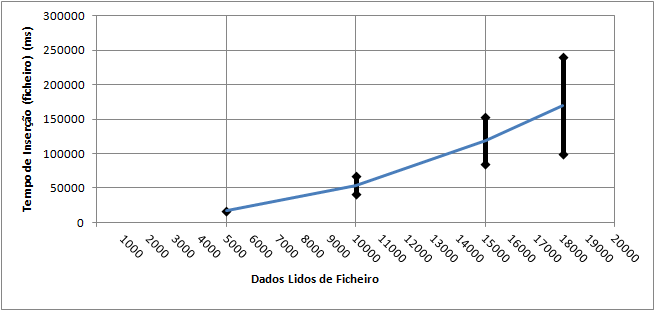
\includegraphics[width=400pt]{cloc_conf1_o1.png}
\end{figure}
\begin{figure}[h!b!t!]
    \caption[Localidades: ArrayList (inserir localidades geradas)]{Localidades: ArrayList (inserir localidades geradas).}
    \label{hashtable}
    \centering
        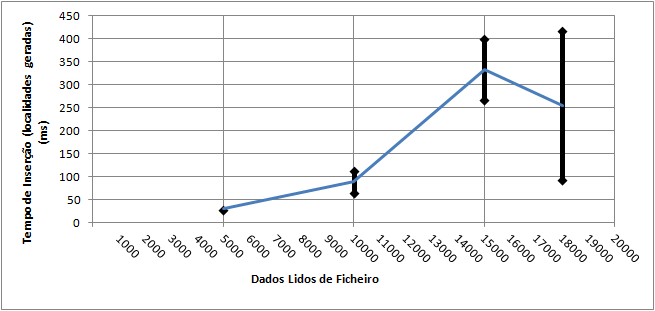
\includegraphics[width=400pt]{cloc_conf1_o2.png}
\end{figure}
\begin{figure}[h!b!t!]
    \caption[Localidades: ArrayList (inserir ligações geradas)]{Localidades: ArrayList (inserir ligações geradas).}
    \label{hashtable}
    \centering
        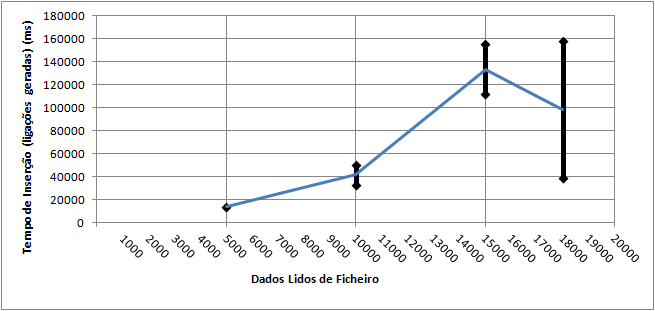
\includegraphics[width=400pt]{cloc_conf1_o3.png}
\end{figure}
\begin{figure}[h!b!t!]
    \caption[Localidades: ArrayList (pesquisar ligações)]{Localidades: ArrayList (pesquisar ligações).}
    \label{hashtable}
    \centering
        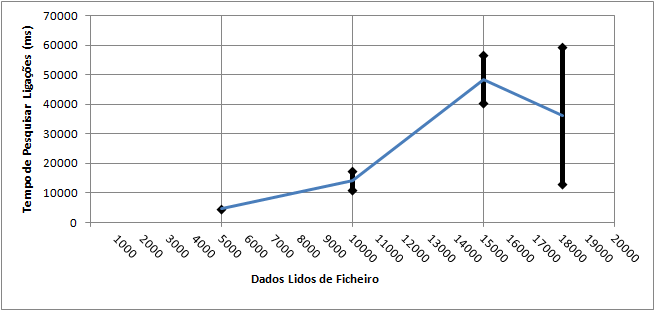
\includegraphics[width=400pt]{cloc_conf1_o4.png}
\end{figure}
\begin{figure}[h!b!t!]
    \caption[Localidades: ArrayList (imprimir dados)]{Localidades: ArrayList (imprimir dados).}
    \label{hashtable}
    \centering
        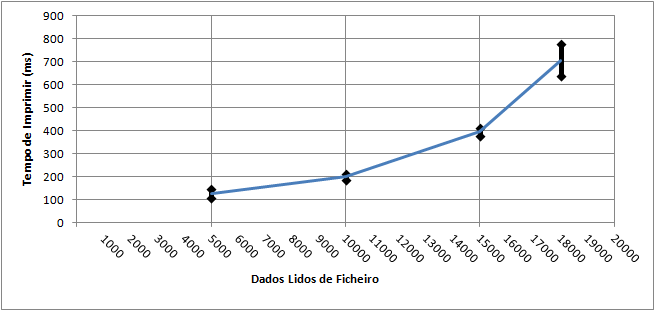
\includegraphics[width=400pt]{cloc_conf1_o5.png}
\end{figure}

\newpage
\twocolumn
\subsubsection[Localidades:\\ArrayList e HashSet]{Localidades: \vbox{ArrayList e HashSet}}
A implementação de ArrayList e HashSet para manusear dados relativos a localidades é uma solução extremamente lenta, à semelhança da implementação anterior (2 ArrayList).

Todos os tempos desta configuração variam de forma próxima à forma linear.
\clearpage
\onecolumn
\begin{center}
    \begin{table}[h!b!t!]
    \begin{center}
    \caption{Tempos da configuração ArrayList e HashSet}
\begin{tabular}{ | *{11}{c|} }
\hline
    Num. & \multicolumn{2}{|c|}{ler ficheiro} & \multicolumn{2}{|c|}{inserir localidades}\\ %\hline
    
    Dados & $\mu$ & $\sigma$ & $\mu$ & $\sigma$\\ \hline
    5000 & 17058.5 & 1347.57 & 29.4 & 2.31\\ \hline
    10000 & 50633.2 & 6373.82 & 87.9 & 24.90\\ \hline
    15000 & 177260.7 & 53279.65 & 216.4 & 58.89\\ \hline
    18000 & 196707.7 & 85599.75 & 225.3 & 107.73\\ \hline
\end{tabular}
\end{center}
\end{table}
\begin{tabular}{ | *{11}{c|} }
\hline
    Num. & \multicolumn{2}{|c|}{inserir ligações} & \multicolumn{2}{|c|}{pesquisar ligações} & \multicolumn{2}{|c|}{escrever}\\ %\hline
    
    Dados & $\mu$ & $\sigma$ & $\mu$ & $\sigma$ & $\mu$ & $\sigma$\\ \hline
    5000 & 14124.2 & 783.79 & 4792.6 & 317.05 & 129.1 & 14.76\\ \hline
    10000 & 41568.4 & 6162.82 & 14034.4 & 1966.17 & 235.7 & 30.72\\ \hline
    15000 & 94508.9 & 23907.09 & 34136.2 & 8907.46 & 483.1 & 61.20\\ \hline
    18000 & 94088.3 & 40083.16 & 33730.2 & 15055.85 & 626.7 & 71.32\\ \hline
\end{tabular}
\end{center}

\begin{figure}[h!b!t!]
    \caption[Localidades: ArrayList e HashSet (ler de ficheiro)]{Localidades: ArrayList e HashSet (ler de ficheiro).}
    \label{hashtable}
    \centering
        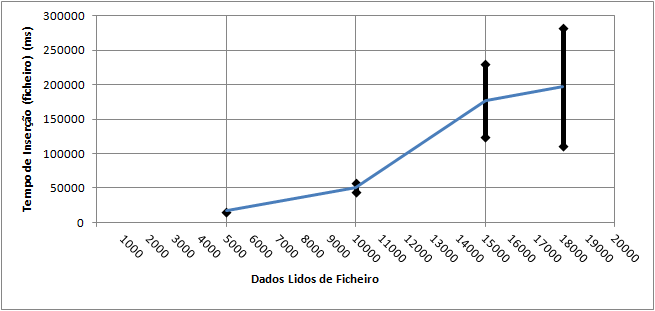
\includegraphics[width=400pt]{cloc_conf2_o1.png}
\end{figure}
\begin{figure}[h!b!t!]
    \caption[Localidades: ArrayList e HashSet (inserir localidades geradas)]{Localidades: ArrayList e HashSet (inserir localidades geradas).}
    \label{hashtable}
    \centering
        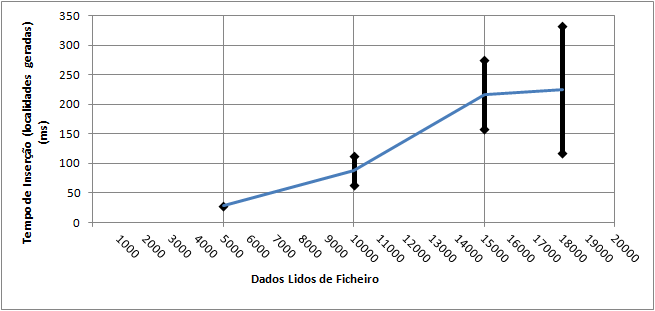
\includegraphics[width=400pt]{cloc_conf2_o2.png}
\end{figure}
\begin{figure}[h!b!t!]
    \caption[Localidades: ArrayList e HashSet (inserir ligações geradas)]{Localidades: ArrayList e HashSet (inserir ligações geradas).}
    \label{hashtable}
    \centering
        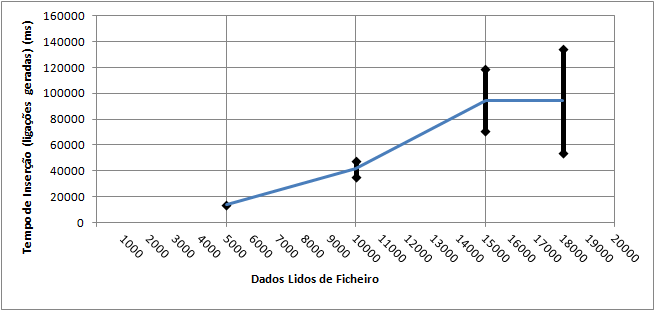
\includegraphics[width=400pt]{cloc_conf2_o3.png}
\end{figure}
\begin{figure}[h!b!t!]
    \caption[Localidades: ArrayList e HashSet (pesquisar ligações)]{Localidades: ArrayList e HashSet (pesquisar ligações).}
    \label{hashtable}
    \centering
        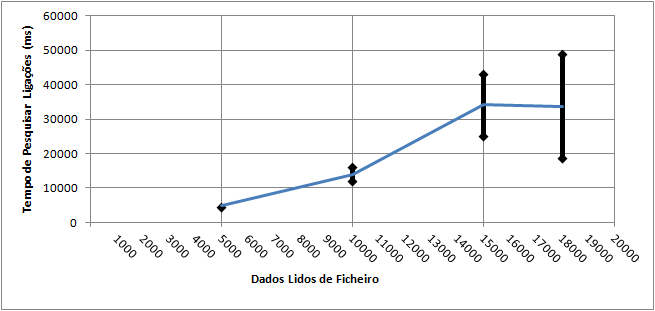
\includegraphics[width=400pt]{cloc_conf2_o4.png}
\end{figure}
\begin{figure}[h!b!t!]
    \caption[Localidades: ArrayList e HashSet (imprimir dados)]{Localidades: ArrayList e HashSet (imprimir dados).}
    \label{hashtable}
    \centering
        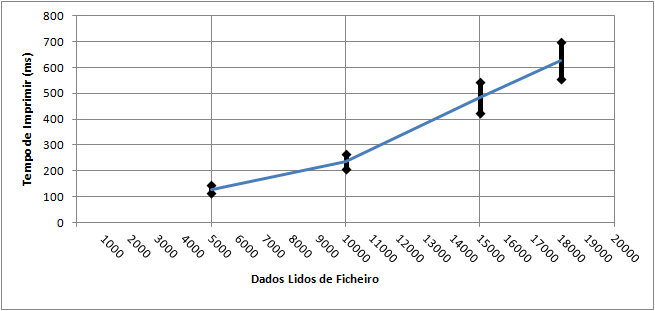
\includegraphics[width=400pt]{cloc_conf2_o5.png}
\end{figure}

\newpage
\twocolumn
\subsubsection{Localidades: HashMap}
A configuração que usa um HashMap para as localidades e um HashMap para as ligações é uma solução muito rápida, comparativamente às anteriores.

Os tempos de inserção de localidades são praticamente constantes e muito próximos de zero. Os tempos de inserção de ligações também aparentam ser constantes e muito próximos dos tempos das pesquisas, de onde se pode concluir que o atraso observado na inserção de ligações deve-se à necessidade de pesquisar a tabela de procura pelo nome da localidade antes de inserir a ligação.

Os tempos da impressão dos dados parecem tomar uma forma exponencial, mas mesmo assim a tabela de procura não deixa de ser rápida, sendo que o seu pior tempo de escrita é de 712ms (quando escreve mais de 18000 localidades e ligações). 
\clearpage
\onecolumn
    \begin{table}[h!b!t!]
    \begin{center}
    \caption{Tempos da configuração HashMap}
\begin{tabular}{ | *{11}{c|} }
\hline
    Num. & \multicolumn{2}{|c|}{ler ficheiro} & \multicolumn{2}{|c|}{inserir localidades} & \multicolumn{2}{|c|}{inserir ligações} & \multicolumn{2}{|c|}{pesquisar ligações} & \multicolumn{2}{|c|}{escrever}\\ %\hline
    
    Dados & $\mu$ & $\sigma$ & $\mu$ & $\sigma$ & $\mu$ & $\sigma$ & $\mu$ & $\sigma$ & $\mu$ & $\sigma$\\ \hline
    5000 & 198.5 & 56.90 & 0.0 & 0.0 & 190.7 & 6.53 & 161.0 & 9.70 & 118.8 & 13.49\\ \hline
    10000 & 225.4 & 12.57 & 0.1 & 0.31 & 188.6 & 1.95 & 171.1 & 24.50 & 257.8 & 36.30\\ \hline
    15000 & 354.4 & 66.65 & 0.1 & 0.31 & 211.1 & 32.29 & 177.3 & 36.13 & 494.3 & 58.44\\ \hline
    18000 & 327.8 & 33.00 & 6.9 & 21.47 & 201.2 & 25.32 & 170.5 & 9.70 & 712.6 & 73.37\\ \hline
\end{tabular}
\end{center}
\end{table}

\begin{figure}[h!b!t!]
    \caption[Localidades: HashMap (ler de ficheiro)]{Localidades: HashMap (ler de ficheiro).}
    \label{hashtable}
    \centering
        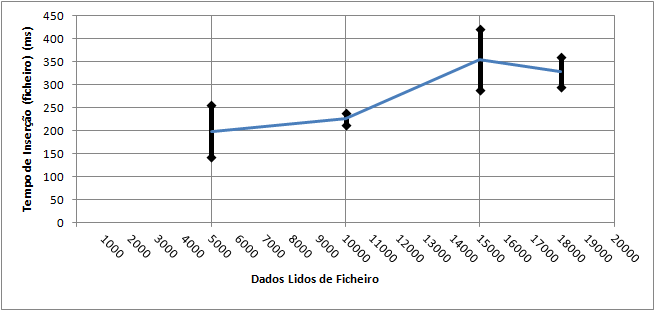
\includegraphics[width=400pt]{cloc_conf3_o1.png}
\end{figure}
\begin{figure}[h!b!t!]
    \caption[Localidades: HashMap (inserir localidades geradas)]{Localidades: HashMap (inserir localidades geradas).}
    \label{hashtable}
    \centering
        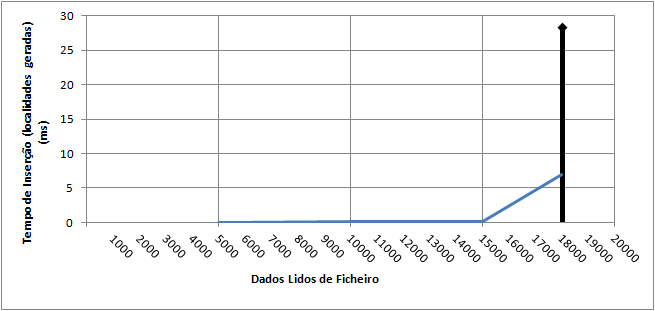
\includegraphics[width=400pt]{cloc_conf3_o2.png}
\end{figure}
\begin{figure}[h!b!t!]
    \caption[Localidades: HashMap (inserir ligações geradas)]{Localidades: HashMap (inserir ligações geradas).}
    \label{hashtable}
    \centering
        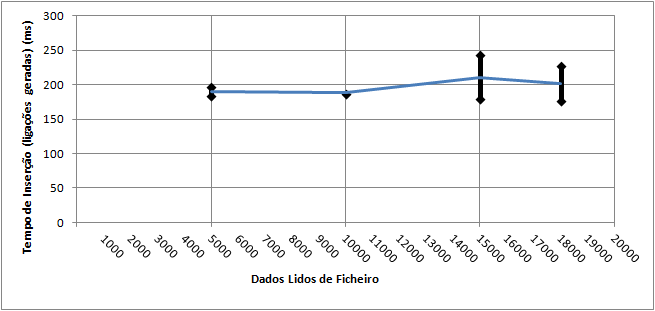
\includegraphics[width=400pt]{cloc_conf3_o3.png}
\end{figure}
\begin{figure}[h!b!t!]
    \caption[Localidades: HashMap (pesquisar ligações)]{Localidades: HashMap (pesquisar ligações).}
    \label{hashtable}
    \centering
        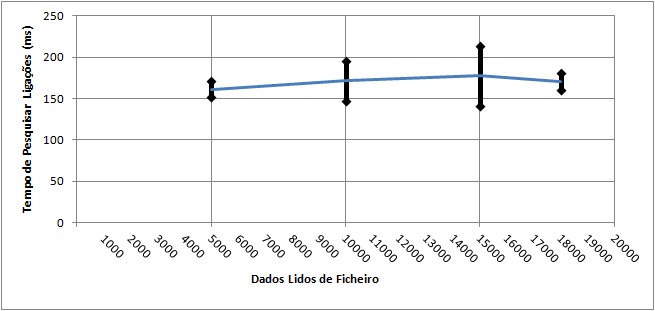
\includegraphics[width=400pt]{cloc_conf3_o4.png}
\end{figure}
\begin{figure}[h!b!t!]
    \caption[Localidades: HashMap (imprimir dados)]{Localidades: HashMap (imprimir dados).}
    \label{hashtable}
    \centering
        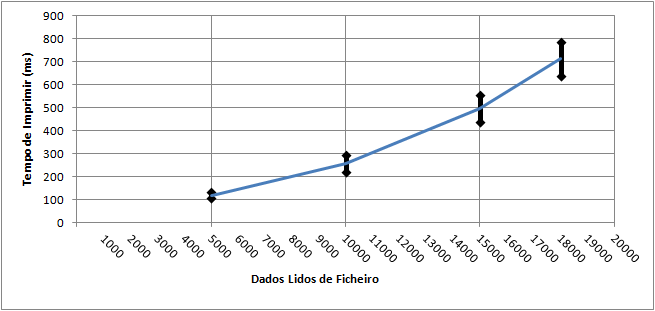
\includegraphics[width=400pt]{cloc_conf3_o5.png}
\end{figure}

\newpage
\twocolumn
\subsubsection{Localidades: TreeMap}
A configuração que usa um TreeMap para as localidades e um TreeMap para as ligações é uma solução muito rápida.

As variações de tempos nos gráficos de tempos da configuração TreeMap são muito semelhantes ao HashMap, excepto que a inserção no TreeMap é mais demorada e segue uma variação linear.

\clearpage
\onecolumn
    \begin{table}[h!b!t!]
    \begin{center}
    \caption{Tempos da configuração TreeMap}
\begin{tabular}{ | *{11}{c|} }
\hline
    Num. & \multicolumn{2}{|c|}{ler ficheiro} & \multicolumn{2}{|c|}{inserir localidades} & \multicolumn{2}{|c|}{inserir ligações} & \multicolumn{2}{|c|}{pesquisar ligações} & \multicolumn{2}{|c|}{escrever}\\ %\hline
    
    Dados & $\mu$ & $\sigma$ & $\mu$ & $\sigma$ & $\mu$ & $\sigma$ & $\mu$ & $\sigma$ & $\mu$ & $\sigma$\\ \hline
    5000 & 228.0 & 10.25 & 0.1 & 0.31 & 222.2 & 18.35 & 175.1 & 8.56 & 130.1 & 25.61\\ \hline
    10000 & 301.5 & 27.84 & 0.2 & 0.42 & 236.1 & 23.40 & 195.4 & 35.85 & 243.4 & 31.66\\ \hline
    15000 & 406.9 & 34.89 & 0.1 & 0.31 & 244.0 & 56.44 & 181.7 & 11.54 & 465.1 & 85.71\\ \hline
    18000 & 470.3 & 56.07 & 0.3 & 0.48 & 231.9 & 17.99 & 174.9 & 17.29 & 670.0 & 36.04\\ \hline
\end{tabular}
\end{center}
\end{table}

\begin{figure}[h!b!t!]
    \caption[Localidades: TreeMap (ler de ficheiro)]{Localidades: TreeMap (ler de ficheiro).}
    \label{hashtable}
    \centering
        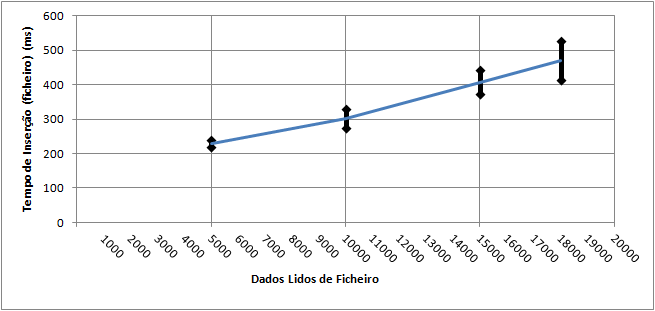
\includegraphics[width=400pt]{cloc_conf4_o1.png}
\end{figure}
\begin{figure}[h!b!t!]
    \caption[Localidades: TreeMap (inserir localidades geradas)]{Localidades: TreeMap (inserir localidades geradas).}
    \label{hashtable}
    \centering
        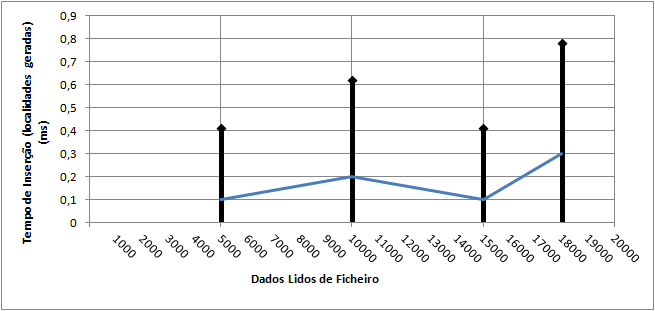
\includegraphics[width=400pt]{cloc_conf4_o2.png}
\end{figure}
\begin{figure}[h!b!t!]
    \caption[Localidades: TreeMap (inserir ligações geradas)]{Localidades: TreeMap (inserir ligações geradas).}
    \label{hashtable}
    \centering
        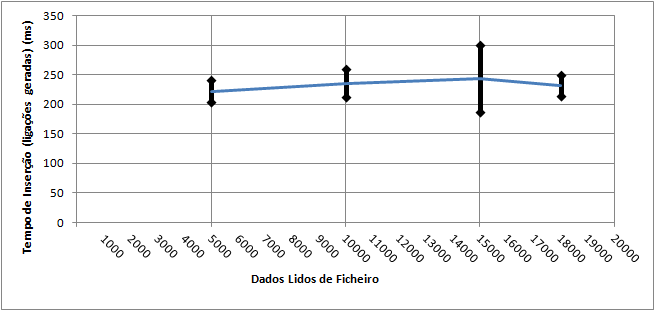
\includegraphics[width=400pt]{cloc_conf4_o3.png}
\end{figure}
\begin{figure}[h!b!t!]
    \caption[Localidades: TreeMap (pesquisar ligações)]{Localidades: TreeMap (pesquisar ligações).}
    \label{hashtable}
    \centering
        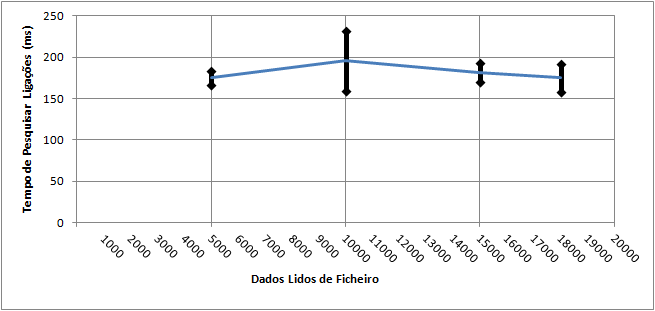
\includegraphics[width=400pt]{cloc_conf4_o4.png}
\end{figure}
\begin{figure}[h!b!t!]
    \caption[Localidades: TreeMap (imprimir dados)]{Localidades: TreeMap (imprimir dados).}
    \label{hashtable}
    \centering
        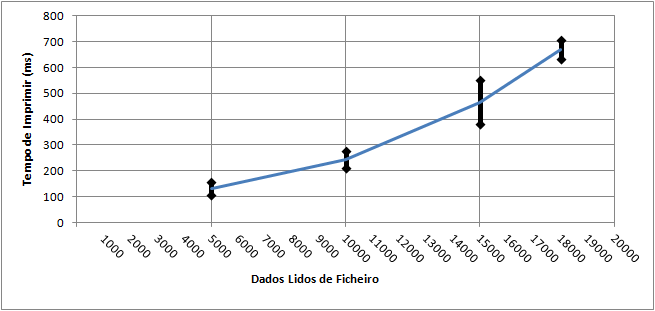
\includegraphics[width=400pt]{cloc_conf4_o5.png}
\end{figure}




\newpage
\twocolumn
\newpage

\subsubsection[Localidades:\\Comparação]{Localidades: Comparação}
De todas as implementações, o ArrayList e o ArrayList com HashSet auxiliar são postos de parte por serem extremamente lentos.

Quanto à escolha entre tabelas de procura e árvores não há dúvidas (como existiram na comparação das implementações para utilizadores). Neste caso o TreeMap não tem qualquer vantagem face ao HashMap.

Assim sendo, conclui-se que a implementação de 2 HashMap é melhor que qualquer outra das implementações cronometradas, no que diz respeito ao manuseamento de Localidades.
\clearpage
\onecolumn
\begin{figure}[h!b!t!]
    \caption[Localidades: Comparação (ler de ficheiro)]{Localidades: Comparação (ler de ficheiro).}
    \label{hashtable}
    \centering
        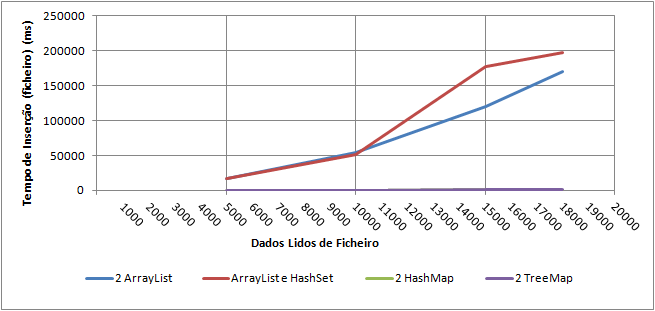
\includegraphics[width=400pt]{cloc_o1.png}
\end{figure}
\begin{figure}[h!b!t!]
    \caption[Localidades: Comparação (inserir localidades geradas)]{Localidades: Comparação (inserir localidades geradas).}
    \label{hashtable}
    \centering
        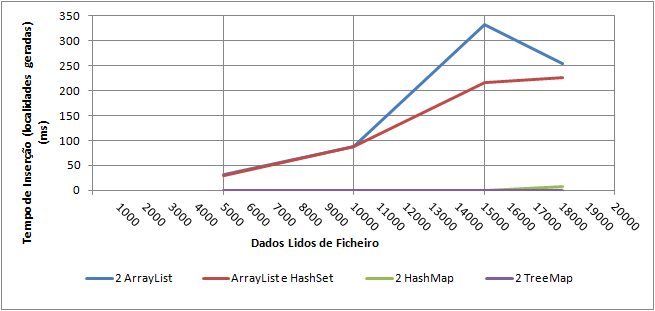
\includegraphics[width=400pt]{cloc_o2.png}
\end{figure}
\begin{figure}[h!b!t!]
    \caption[Localidades: Comparação (inserir ligações geradas)]{Localidades: Comparação (inserir ligações geradas).}
    \label{hashtable}
    \centering
        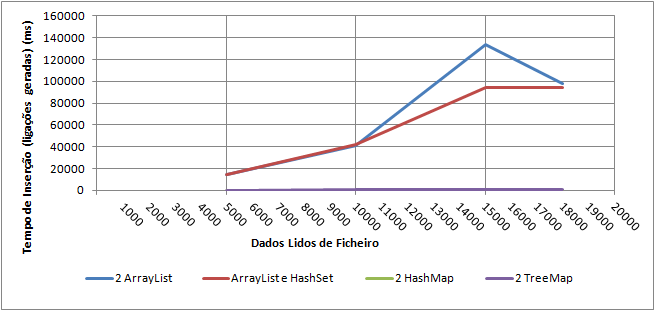
\includegraphics[width=400pt]{cloc_o3.png}
\end{figure}
\begin{figure}[h!b!t!]
    \caption[Localidades: Comparação (pesquisar ligações)]{Localidades: Comparação (pesquisar ligações).}
    \label{hashtable}
    \centering
        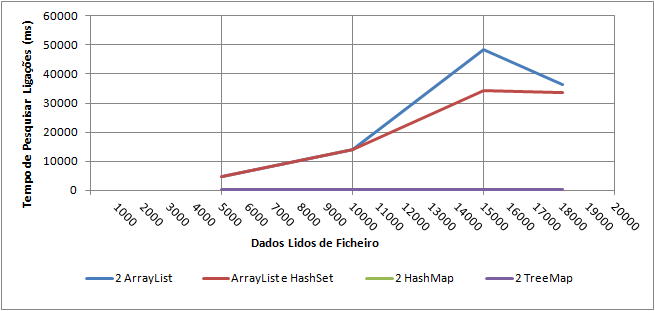
\includegraphics[width=400pt]{cloc_o4.png}
\end{figure}
\begin{figure}[h!b!t!]
    \caption[Localidades: Comparação (imprimir dados)]{Localidades: Comparação (imprimir dados).}
    \label{hashtable}
    \centering
        \includegraphics[width=400pt]{cloc_o5.png}
\end{figure}


\clearpage
\section{Conclusão}
Depois da criação de uma aplicação de testes de desempenho e da avaliação dos resultados produzidos pela aplicação, chega-se à conclusão que a melhor implementação para ambos Utilizadores e Localidades é o HashMap.

Mesmo sendo ligeiramente menos eficiente no que diz respeito à listagem dos seus elementos, o HashMap mantém os melhores tempos de inserção e procura de dados. Assim sendo é a implementação escolhida para manuseamento de Utilizadores e Localidades.

\clearpage
\onecolumn
\section{Fotos}
\begin{center}
    \begin{tabular}{ccc}
        \includegraphics[width=90pt]{bruno.png}&
        \includegraphics[width=90pt]{daniel.png}\\
        
        \small{\textbf{Bruno Ferreira}}&
        \small{\textbf{Daniel Carvalho}}\\
        \small{\textbf{A61055}}&
        \small{\textbf{A61008}}\\
    \end{tabular}
\end{center}
\end{document}